\documentclass[border=3.14mm]{standalone}

\usepackage{tikz}
\usepackage{ifthen}
\usetikzlibrary{math}
\begin{document}
\pagestyle{empty}

\pgfdeclarelayer{background}
\pgfsetlayers{background,main}

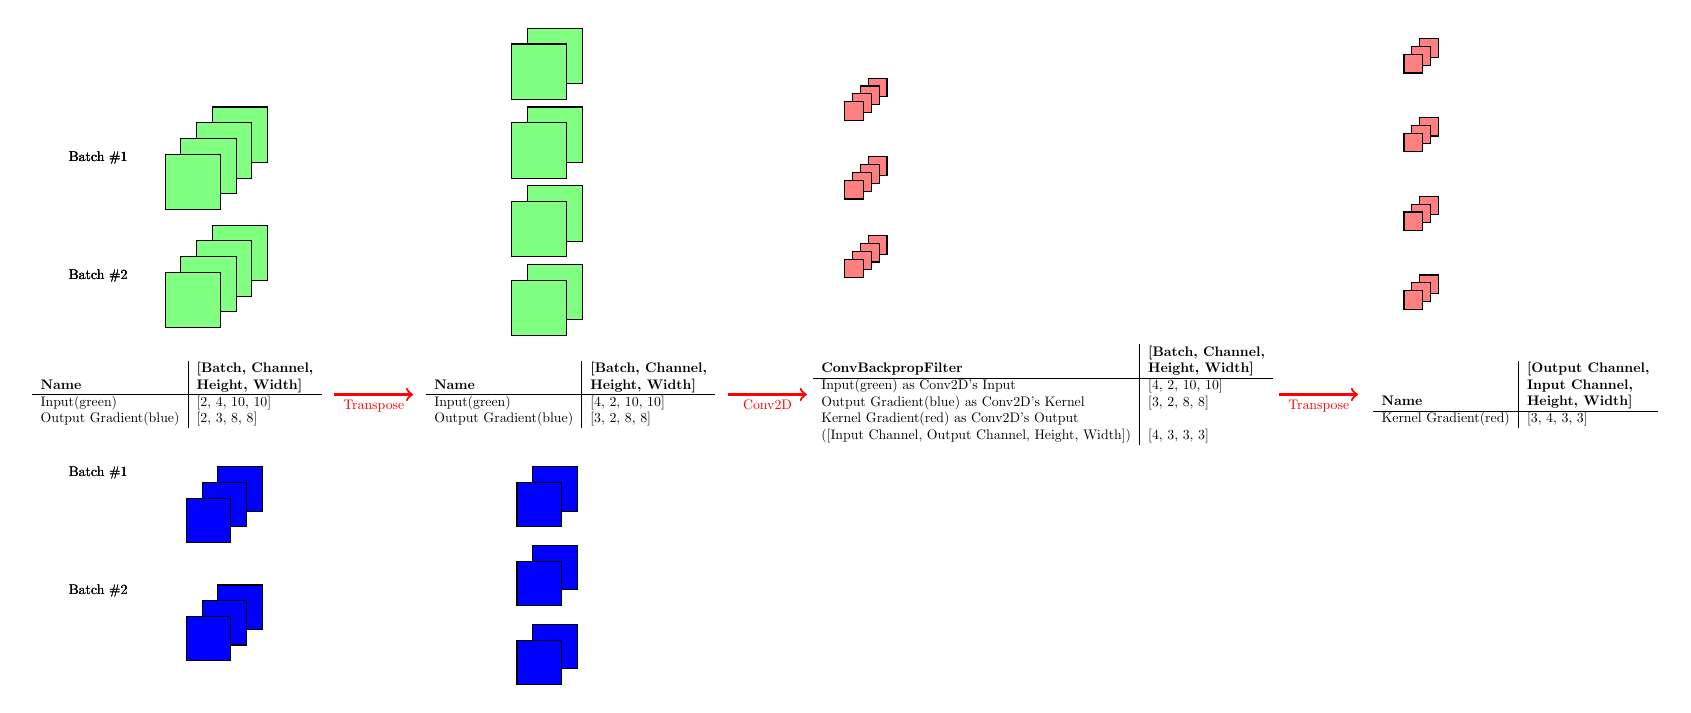
\begin{tikzpicture}[draw=black!50]
\tikzstyle{neuron}=[rectangle, draw=black, fill=black!25]
\tikzstyle{input neuron}=[neuron, fill=green!50, minimum size=20pt];
\tikzstyle{output neuron}=[neuron, fill=blue, minimum size=16pt];
\tikzstyle{kernel neuron}=[neuron, fill=red!50, minimum size=6pt];
\tikzstyle{kline} = [red, thick]

% Draw the input layer nodes
\tikzmath{
    \batchsize = 2;
    \inputsize = 4;
    \outputsize = 3;
}

\foreach \bn in {1,...,\batchsize}
    \foreach \x in {1,...,\inputsize} {
        \tikzmath{
            real \bshift;
            \bshift = -3 * \bn - 1;
        }
        \node[scale=0.5, yshift = \bshift cm] () {Batch \#\bn};
        \node[input neuron, xshift=2cm, yshift = \bn * -1.5cm] () at (-\x * 0.2, -\x * 0.2) {};
    };

\foreach \bn in {1,...,\batchsize}
    \foreach \x in {1,...,\outputsize} {
        \tikzmath{
            real \bshifta, \bshiftb;
            \bshifta = -3 * \bn - 1 - 8;
            \bshiftb = \bn * -1.5 - 4.5;
        }
        \node[scale=0.5, yshift = \bshifta cm] () {Batch \#\bn};
        \node[output neuron, xshift=2cm, yshift = \bshiftb cm] () at (-\x * 0.2, -\x * 0.2) {};
    };

\draw [->, kline] (3, -5) -- node[scale=0.5, anchor=north] {Transpose} (4, -5);

\foreach \x in {1,...,\inputsize}
    \foreach \bn in {1,...,\batchsize} {
        \tikzmath{
            real \bshifta;
            \bshifta = -1 * \x + 0.5;
        }
        \node[input neuron, xshift=6cm, yshift = \bshifta cm] () at (-\bn * 0.2, -\bn * 0.2) {};
    };

\foreach \x in {1,...,\outputsize}
    \foreach \bn in {1,...,\batchsize} {
        \tikzmath{
            real \bshifta;
            \bshifta = -1 * \x - 5;
        }
        \node[output neuron, xshift=6cm, yshift = \bshifta cm] () at (-\bn * 0.2, -\bn * 0.2) {};
    };

\node [scale=0.5, xshift=2cm, yshift=-10cm](LegendTable) {
    \begin{tabular}{l|l} 
     & \textbf{[Batch, Channel,} \\
    \textbf{Name} & \textbf{Height, Width]} \\
    \hline
    Input(green) & [2, 4, 10, 10] \\
    Output Gradient(blue) & [2, 3, 8, 8] \\
    \end{tabular}
};

\node [scale=0.5, xshift=12cm, yshift=-10cm](LegendTable) {
    \begin{tabular}{l|l} 
     & \textbf{[Batch, Channel,} \\
    \textbf{Name} & \textbf{Height, Width]} \\
    \hline
    Input(green) & [4, 2, 10, 10] \\
    Output Gradient(blue) & [3, 2, 8, 8] \\
    \end{tabular}
};

\draw [->, kline] (8, -5) -- node[scale=0.5, anchor=north] {Conv2D} (9, -5) ;

\foreach \x in {1,...,\outputsize}
    \foreach \y in {1,...,\inputsize} {
        \tikzmath{
            real \bshifta;
            \bshifta = -1 * \x;
        }
        \node[kernel neuron, xshift=10cm, yshift=\bshifta cm] () at (-\y * 0.1, -\y * 0.1) {};
    };

\node [scale=0.5, xshift=24cm, yshift=-10cm](LegendTable) {
    \begin{tabular}{l|l} 
     & \textbf{[Batch, Channel,} \\
    \textbf{ConvBackpropFilter} & \textbf{Height, Width]} \\
    \hline
    Input(green) as Conv2D's Input & [4, 2, 10, 10] \\
    Output Gradient(blue) as Conv2D's Kernel & [3, 2, 8, 8] \\
    Kernel Gradient(red) as Conv2D's Output & \\
    ([Input Channel, Output Channel, Height, Width]) & [4, 3, 3, 3] \\
    \end{tabular}
};

\draw [->, kline] (15, -5) -- node[scale=0.5, anchor=north] {Transpose} (16, -5) ;

\foreach \x in {1,...,\inputsize}
    \foreach \y in {1,...,\outputsize} {
        \tikzmath{
            real \bshifta;
            \bshifta = -1 * \x + 0.5;
        }
        \node[kernel neuron, xshift=17cm, yshift=\bshifta cm] () at (-\y * 0.1, -\y * 0.1) {};
    };

\node [scale=0.5, xshift=36cm, yshift=-10cm](LegendTable) {
    \begin{tabular}{l|l} 
     & \textbf{[Output Channel,} \\
     & \textbf{Input Channel,} \\
    \textbf{Name} & \textbf{Height, Width]} \\
    \hline
    Kernel Gradient(red) & [3, 4, 3, 3] \\
    \end{tabular}
};

\end{tikzpicture}
% End of code
\end{document}
